\section[TEM]{Transmissionenelektronenmikroskop} % (fold)
\label{sec:tem}
\subsection*{subsection name} % (fold)
\label{sub:subsection_name}

\begin{frame}
	\frametitle{Elektronenmikroskopie}
	\begin{figure}
		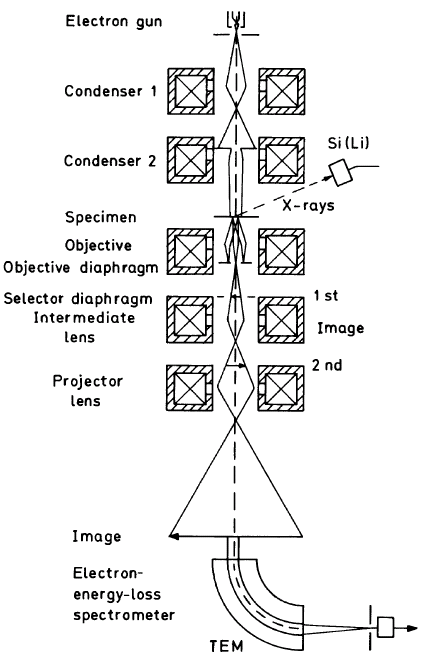
\includegraphics[height = 7.5cm]{pic/tem.png}
	\end{figure}
\end{frame}
% subsection subsection_name (end)
\begin{frame}
	\frametitle{Elektronenmikroskopie}
	\begin{block}{Elektronenquelle}
		\begin{itemize}
			\item Thermische Elektronen
			\item Schottky-Diode
			\item Feldemissionsquelle
		\end{itemize}
	\end{block}
	\begin{figure}
		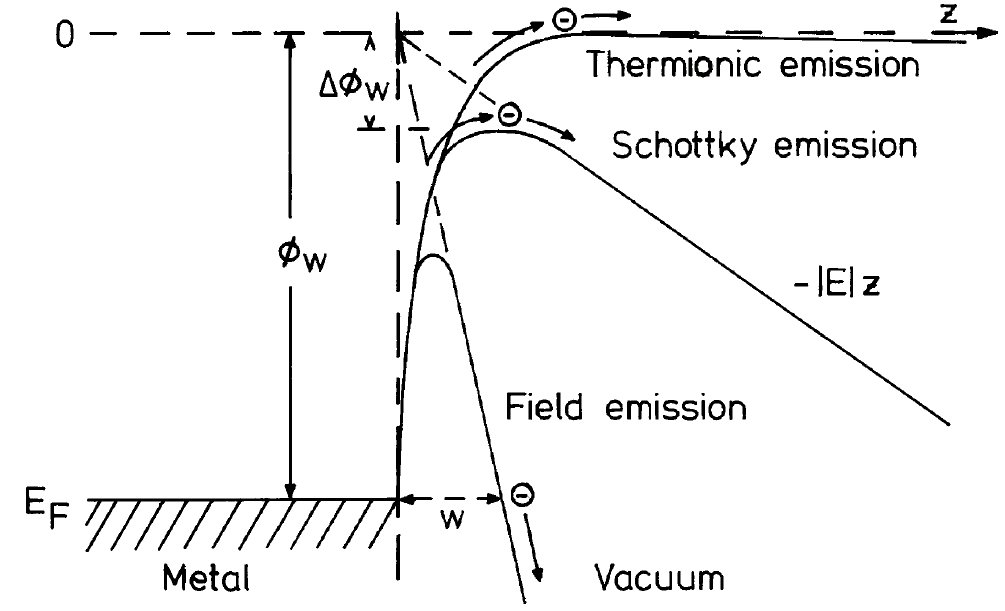
\includegraphics[height = 5cm]{pic/emission.png}
	\end{figure}
\end{frame}

\begin{frame}
	\frametitle{Elektronenmikroskopie}
	\begin{block}{Linsen}
		\begin{itemize}
			\item Kondensorsystem
			\item Objektsystem
		\end{itemize}
	\end{block}
	\begin{figure}
		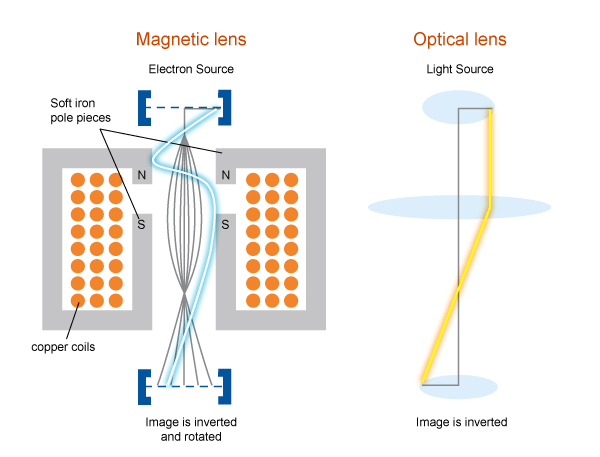
\includegraphics[height = 5.5cm]{pic/lens.png}
	\end{figure}
\end{frame}

\begin{frame}
	\frametitle{Elektronenmikroskopie}
	\begin{block}{Filter}
		\begin{itemize}
			\item Kontrastblenden
			\item Omega Energiefilter
		\end{itemize}		
	\end{block}
\end{frame}

\begin{frame}
	\frametitle{Elektronenmikroskopie}
	\begin{figure}
		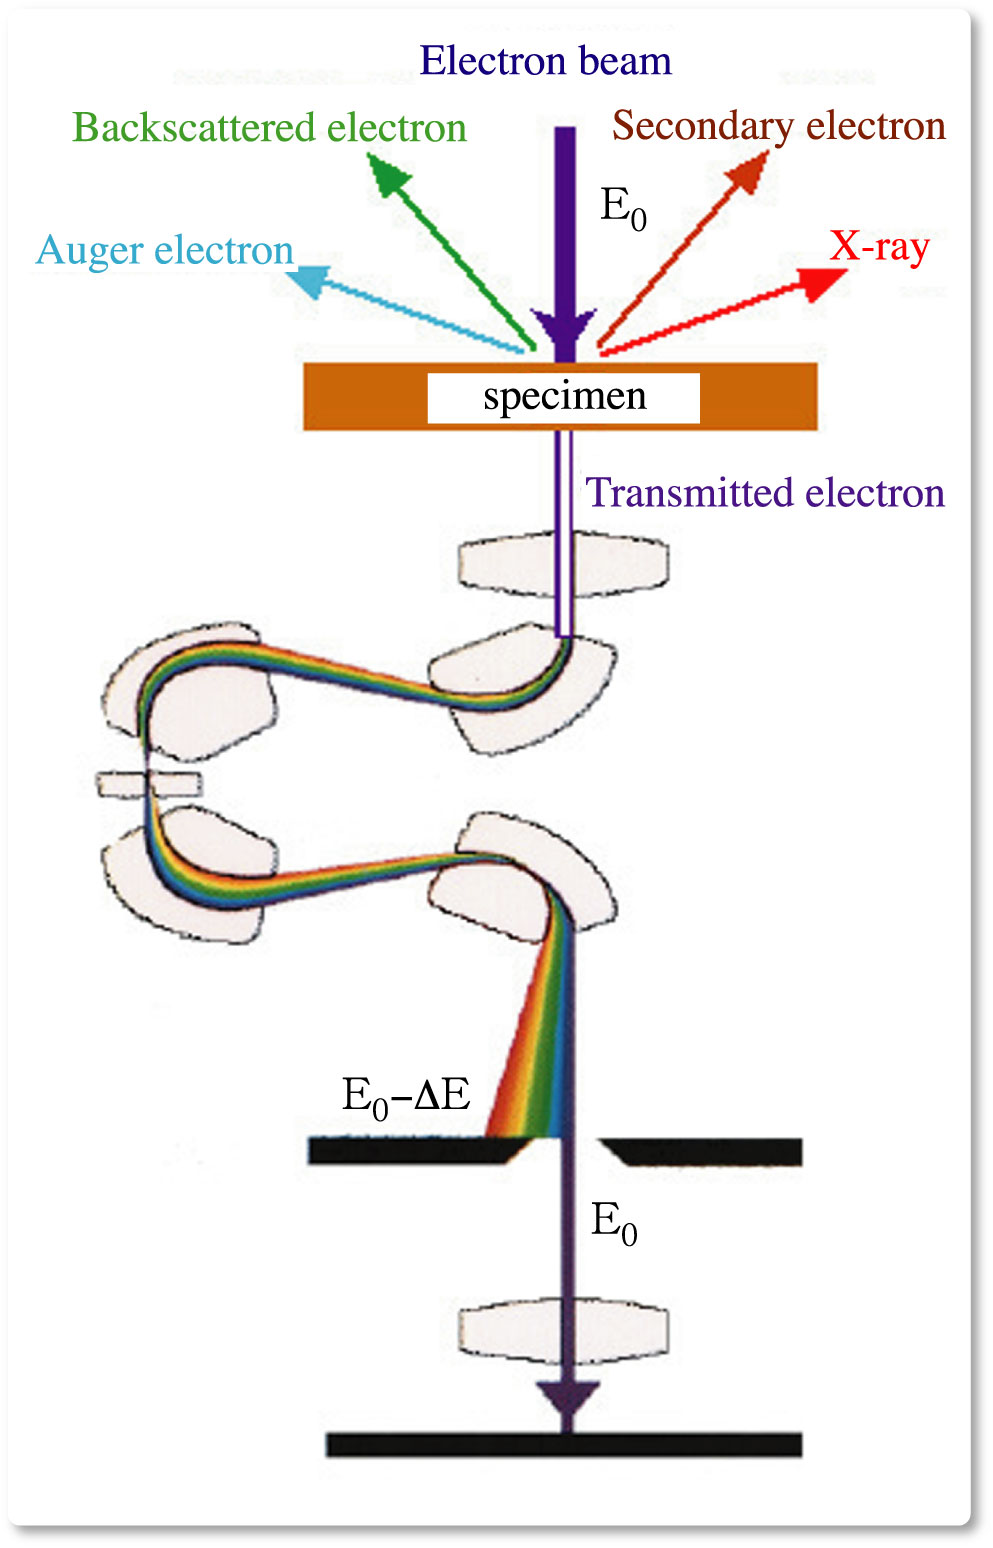
\includegraphics[height = 8cm]{pic/omega.jpg}
	\end{figure}
\end{frame}

\begin{frame}
	\frametitle{Elektronenmikroskopie}
	\begin{block}{Detektoren}
		\begin{itemize}
			\item Fluoreszensschirm
			\item CCD - Kameras
			\item Direkte Elektronen Detektion
		\end{itemize}
	\end{block}
	\begin{figure}
		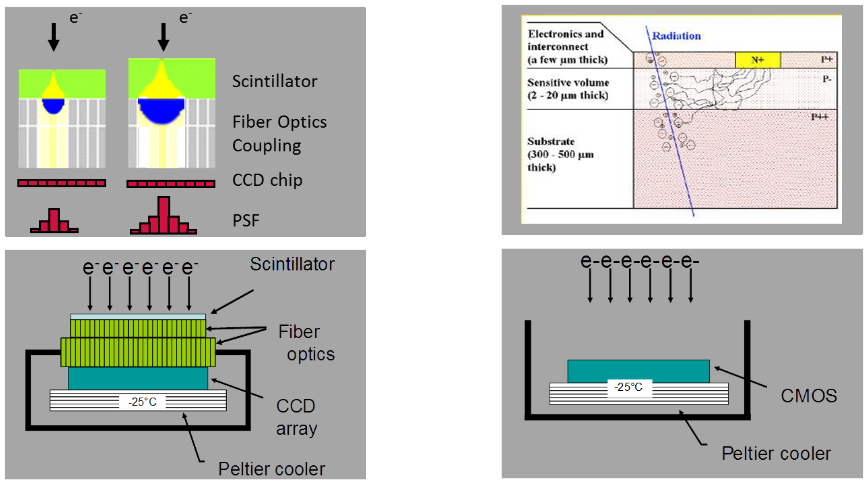
\includegraphics[height = 5cm]{pic/ccd.png}
	\end{figure}
\end{frame}

\begin{frame}
	\frametitle{Elektronenmikroskopie}
	\begin{block}{Bildfehler}
		\begin{itemize}
			\item Drift
			\item Astigmatismus (Objekt, Kondensor)
			\item Rauschen
		\end{itemize}
	\end{block}
	\begin{figure}
		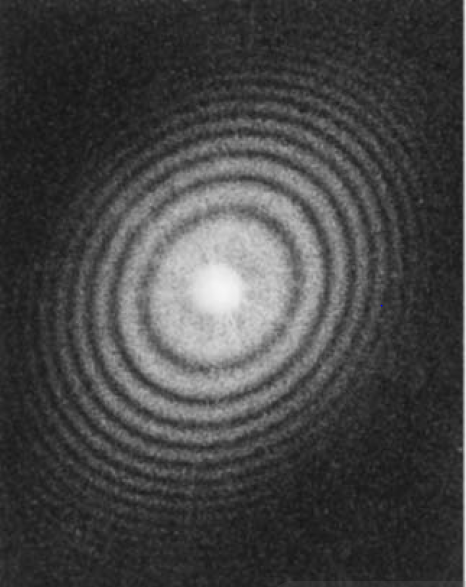
\includegraphics[width = 4cm]{pic/astigmatismus.png}
	\end{figure}
\end{frame}

\begin{frame}
	\frametitle{Elektronenmikroskopie}
	\begin{block}{Auflösungsvermögen}
		\begin{itemize}
			\item Wellenlänge
			\item Abbe Kriterium
			\item Größe der Pixel
			\item Bildfehler
		\end{itemize}
	\end{block}
	\begin{equation*}
		\text{Auflösung}_{\text{max}} = 2 \cdot \frac{\text{Pixelgröße}}{\text{Vergrößerung}}
	\end{equation*}
\end{frame}